\documentclass[12pt,twoside,a4paper]{report}
\usepackage{amsmath}
\usepackage{amssymb}
\usepackage{graphicx}
\usepackage{fancyhdr}
\usepackage{enumerate}
\usepackage[vmargin=2.5cm, hmargin=2.5cm]{geometry}
\usepackage{hyperref}
\usepackage{fontspec}
\usepackage{unicode-math}
\usepackage{stackengine}
\usepackage{minitoc}
\usepackage{amsthm}
\usepackage{listings}
\usepackage{xcolor}
\usepackage{xeCJK}


\setmainfont{Linux Libertine O}
\setsansfont{Linux Biolinum O}
\setCJKmainfont{Noto Serif CJK JP}

\graphicspath{{./fig/category_theory/}{./fig/agda/lagda/latex/}}

\setlength{\parindent}{0em}
\addtolength{\parskip}{1ex}

\usepackage[backend=biber,style=ieee]{biblatex}
\addbibresource{ref.bib}

\theoremstyle{definition}
\newtheorem*{definition*}{Definition}

\theoremstyle{definition}
\newtheorem*{theorem*}{Theorem}

\newcounter{motivation}
\renewcommand{\themotivation}{\Roman{motivation}}

\newcommand{\motivation}[1]{%
    \refstepcounter{motivation}%
    \vspace{1.5em}%
    \noindent\textbf{Motivation \themotivation.  #1}
    \par
    \expandafter\edef\csname savedmotivation\themotivation\endcsname{%
        \noexpand\noindent\noexpand\textbf{Motivation \themotivation. #1}\noexpand\par
    }%
}

\newcommand{\secref}[1]{\S\ref{#1}}

\definecolor{mediumblue}{HTML}{0000CD}
\definecolor{green}{HTML}{008B00}
\newcommand{\mb}[1]{\textcolor{mediumblue}{#1}}
\newcommand{\gn}[1]{\textcolor{green}{#1}}

\newcommand{\bN}{\mathbb{N}}

\newcommand{\yo}{\mathord{\text{\kern0.03em \scalebox{0.8}{よ}\kern0.03em}}}

\begin{document}

\dominitoc

\title{Using functor categories to generate intermediate code with Agda}
\author{Jack Gao}
\date{\today}
\maketitle

\tableofcontents
\newpage

\chapter{Introduction}
    \minitoc
    An Algol-like language is a typed lambda calculus with store. In this dissertation, the source language is an Algol-like language with the following primitive types:
    \begin{itemize}
        \item 
            \textbf{comm}: the commands
        \item 
            \textbf{intexp}: the integer expressions
        \item 
            \textbf{intacc}: the integer acceptors
        \item 
            \textbf{intvar}: the integer variables
    \end{itemize}
    and the set $\Theta$ of types is defined as follows:
    \[ \Theta := \textbf{comm} \mid \textbf{intexp} \mid \textbf{intacc} \mid \textbf{intvar} \mid \Theta \to \Theta \]

    [Considering adding an example of Algol-like language here]

    The target language is an assembly-style intermediate language for a stack machine. It is defined with four stack-descriptor-indexed families of non-terminals: 
    \begin{itemize}
        \item 
            $\langle\text{L}_{sd}\rangle$: lefthand sides
        \item 
            $\langle\text{S}_{sd}\rangle$: Simple righthand sides
        \item
            $\langle\text{R}_{sd}\rangle$: righthand sides
        \item
            $\langle\text{I}_{sd}\rangle$: instruction sequences
    \end{itemize}

    The grammer of the target language is specified in Chapter 3. [Add exact section/subsection here]

    This dissertation presents an implementation of a compiler from the source language to the target language with Agda \cite{Agda}. This implementation is based on the work of Reynolds \cite{Reynolds}, who presented a denotational semantics of Algol-like languages in the form of a presheaf category over stack descriptors. The compiler is implemented as a functor from the source language to the target language. The implementation is verified with Agda's type system, which ensures that the generated code is well-typed and adheres to the semantics of both the source and target languages. This implementation proves and refines Reynolds' work, providing a practical example of how to use functor categories to generate intermediate code.

    \section{Motivation and related work} \label{sec: motivation}
        The denotational semantics of Algol-like languages can be structured as a presheaf category over stack descriptors, which has been shown by Reynolds \cite{essence} and Oles \cite{Oles_1} \cite{Oles_2}. By interpreting the source language into this category, where objects of the category represent instruction sequences parameterised by stack layouts, the semantic model directly yields a compiler. The mathematical structure of the compiler has been specified by Reynolds in his paper ``Using Functor Categories to Generate Intermediate Code'' \cite{Reynolds}.

        This project is motivated and guided by the following:

        \motivation{Implementation of the compiler}
        Reynolds concluded that he did not have a proper dependently typed programming language in hand, so his compiler remained a partial function theoretically. We aim to provide a computer implementation of this theoretical framework in a dependently typed programming language.
        

        \motivation{Formal verification of the compiler}
        The terms in Reynolds' work are also written by hand. Terms are complicated and error-prone, and it is difficult to verify the correctness of the terms. We aim to provide a formalisation of the terms in a proof assistant to verify the correctness of the terms.
        
        \motivation{Trend of verified compilers}
        The rise of verified compilers including CompCert \cite{CompCert}, CakeML \cite{CakeML} reflects a broader trend toward trustworthy systems, where correctness proofs replace testing for critical guarantees. Like Lean 4 \cite{Lean4}, we leverage dependent types to internalise the verification of correctness of terms.

    
    \section{Language choice: Agda's advantages}
        Agda \cite{Agda} is a dependently typed programming language and proof assistant. Agda captures the source language's intrinsic sytax with indexed families, which contains only well-typed terms. Therefore, it focuses on the correct programs and rules out the ill-typed nonsensical inputs. 

        Dependently typed languages provide a natural framework for expressing functor categories is proven both theoretically and practically. There have been dependent-type-theoretic model of categories \cite{Dybjer}, and it has been shown that functor categories arise naturally as dependent function types \cite{Jacobs}. A formalisation of Category Theory, including cartesian closed categories, functors and presheaves has been developed in Agda by Hu and Caratte \cite{Cat_Agda}. Other proof assistants, such as Isabelle/Hol, does not have a dependently typed language structure, and thus cannot express the functor categories as naturally as Agda. Agda also provides an interactive environment for writing and verifying programs, which will be further discussed in \secref{subsec: holes}.

        [Do I need a table for comparing other proof assistants and Agda?]


    \section{Contributions}
        Addressed the three motivations presented in \secref{sec: motivation} and contributed to the following:
        \begin{quote}
            \savedmotivationI
            We implemented the compiler from the source language to the target language in Agda. 

            \savedmotivationII
            We formalised the terms in the source language and target language in Agda, and proved that the compiler is a functor from the source language to the target language. 

            \savedmotivationIII
            This implementation follows the trend of verified compilers, and provides a practical example of how to use functor categories to generate intermediate code.
        \end{quote}


\chapter{Preparation}
    \minitoc

    \section{Starting Point}
    Prior to this project, I had no experience with Agda. Although I was aware of the open-source online tutorial \textit{Programming Language Foundations in Agda} (PLFA) \cite{plfa}, my preparation was limited to setting up the Agda environment on my laptop by following the ``Front Matter'' section of the tutorial.

    I did not have any other experience with compiler beyond Part IB Compiler Construction Course. I had no prior exposure to category theory and type theory before the Part II lectures.


    \section{Category theory background} \label{sec: cat}
        Category theory provides a high-level abstraction from which we can reason about the structure of mathematical objects and their relationships. It provides us a ``bird's eye view'' of the mathematics which enable us to spot patterns that are difficult to see in the details. \cite{basic_cat} More specifically, it provides a ``purer'' view of functions that is not derived from sets. \cite{scott-lambda} Compared to set theory which is ``element-oriented'', category theory is ``function-oriented'' and ``morphism-oriented''. We understand structures not via elements but by how they transform into each other. 

        Notation in category theory is similar to that in set theory and type theory. For example, $A, B, \dots$ are used to denote objects, sets, or types, and arrows are used to denote morphisms or functions (e.g.\ $A \to B$). There is a deeper connection between category theory and type theory. Curry-Howard correspondence \cite{curry-howard} states that there is a correspondence between logic and type theory, where propositions correspond to types and proofs correspond to terms. This correspondence was later extended by Joachim Lambek, who showed that cartesian closed categories provide a natural semantic setting for the simply typed lambda calculus. \cite{lambek} Under this perspective, types become objects in a category, and programs correspond to morphisms. We will further explore this connection in \secref{subsec: curry-howard-lambek}.


        The following is a brief introduction to the basic concepts of category theory, which is based on the work of Leinster \cite{basic_cat}, 
        Riehl \cite{cat_context}, and the lecture notes of Part II Category Theory by Andrew Pitts and Marcelo Fiore \cite{cat_lecture_notes}.

        \subsection{Category}
        \begin{definition*}[Category]
            A \emph{category} $\mathcal{C}$ is specified by the following:
            \begin{itemize}
                \item 
                    a collection of objects $\textbf{obj}(\mathcal{C})$, whose elements are called $\mathcal{C}$-objects;
                \item 
                    for each $X, Y \in \textbf{obj}(\mathcal{C})$, a collection of morphisms $\mathcal{C}{(X,Y)}$, whose elements are called $\mathcal{C}$-morphisms from $X$ to $Y$ (e.g.\ $f : X \to Y$);
                \item 
                    for each $X \in \textbf{obj}(\mathcal{C})$, an element $\textbf{id}_X \in \mathcal{C}{(X,X)}$ called the identity morphism on $X$;
                \item 
                    for each $X, Y, Z \in \textbf{obj}(\mathcal{C})$, a function 
                    \[\begin{aligned}
                        \mathcal{C}{(X,Y)} \times \mathcal{C}{(Y,Z)} &\to \mathcal{C}{(X,Z)} \\
                        (f,g) &\mapsto g \circ f
                    \end{aligned}\]
                    called the composition of morphisms;
            \end{itemize}
            satisfying the following properties:
            \begin{itemize}
                \item 
                    \textbf{(Unit Laws)}
                    for all $X, Y \in \textbf{obj}(\mathcal{C})$ and $f \in \mathcal{C}{(X,Y)}$, we have:
                    \begin{equation} \label{law: unit}
                        \textbf{id}_Y \circ f = f = f \circ \textbf{id}_X
                    \end{equation}
                \item
                    \textbf{(Associativity Law)}
                    for all $X, Y, Z, W \in \textbf{obj}(\mathcal{C})$ and $f \in \mathcal{C}{(X,Y)}$, $g \in \mathcal{C}{(Y,Z)}$, $h \in \mathcal{C}{(Z,W)}$, we have:
                    \begin{equation} \label{law: associativity}
                        h \circ (g \circ f) = (h \circ g) \circ f
                    \end{equation}
            \end{itemize}
        \end{definition*}

        An example of category is the category of sets, denoted as $\mathcal{Set}$, specifed by:
        \begin{itemize}
            \item 
                the objects of $\mathcal{Set}$ are a fixed universe of sets;
            \item
                for each $X, Y \in \textbf{obj}(\mathcal{Set})$, the morphisms from $X$ to $Y$ in $\mathcal{Set}$ are the functions from $X$ to $Y$;
            \item
                the identity morphism on $X$ in $\mathcal{Set}$ is the identity function on $X$;
            \item
                the composition of morphisms in $\mathcal{Set}$ is defined as the composition of functions.
        \end{itemize}
        Associativity law and unit laws are satisfied in $\mathcal{Set}$, since the composition of functions is associative and the identity function compose with any function is the function itself.

            \subsubsection{Opposite category}
            The idea of opposite category is that if we have a category $\mathcal{C}$, we can reverse the direction of all morphisms in $\mathcal{C}$ to obtain a new category $\mathcal{C}^{\textbf{op}}$.

            \begin{definition*}[Opposite category]
                Given a category $\mathcal{C}$, its \emph{opposite category} $\mathcal{C}^{\textbf{op}}$ is specified by:
                \begin{itemize}
                    \item 
                        the objects of $\mathcal{C}^{\textbf{op}}$ are the same as those of $\mathcal{C}$;
                    \item 
                        for each $X, Y \in \textbf{obj}(\mathcal{C})$, the morphisms from $X$ to $Y$ in $\mathcal{C}^{\textbf{op}}$ are the morphisms from $Y$ to $X$ in $\mathcal{C}$;
                    \item 
                        the identity morphism on $X$ in $\mathcal{C}^{\textbf{op}}$ is the identity morphism on $X$ in $\mathcal{C}$;
                    \item 
                        the composition of morphisms in $\mathcal{C}^{\textbf{op}}$ is defined as the composition of morphisms in $\mathcal{C}$.
                \end{itemize}
            \end{definition*}

                % \paragraph{The principle of duality}
                % Whenever one defines a concept or proves a theorem in category theory $\mathcal{C}$, one can obtain another concept or theorem in the opposite category $\mathcal{C}^{\textbf{op}}$, called the \emph{dual} of the original concept or theorem, by reversing all arrows in the original concept or theorem.

            The notation of commutative diagram is widely used in category theory as a convenient visual representation of the relationships between objects and morphisms in a category.
            \subsubsection{Commutative diagrams}
            A \emph{diagram} in a category $\mathcal{C}$ is a directed graph whose vertices are $\mathcal{C}$-objects and whose edges are $\mathcal{C}$-morphisms.

            A diagram is \emph{commutative} (or \emph{commutes}) if any two finite paths in the graph between any two vertices $X$ and $Y$ in the diagram determine the equal morphism $f \in \mathcal{C}{(X,Y)}$ under the composition of morphisms.

            \begin{figure}[htb!]
                \centering
                \begin{minipage}{0.3\textwidth}
                    \centering
                    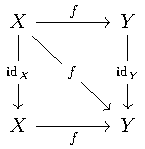
\includegraphics[width=0.8\textwidth]{unit_laws.pdf}
                    \caption{Commutative diagram for Unit Laws}
                    \label{fig: unit_laws}
                \end{minipage} \hspace{0.2\textwidth}
                \begin{minipage}{0.3\textwidth}
                    \centering
                    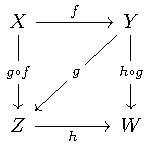
\includegraphics[width=0.8\textwidth]{associativity_law.pdf}
                    \caption{Commutative diagram for Associativity Law}
                    \label{fig: associativity_law}
                \end{minipage}
            \end{figure}

            As examples of commutative diagrams, Figure \ref{fig: associativity_law} and Figure \ref{fig: unit_laws} are commutative diagrams for the unit laws and associativity law respectively. 

        
        \subsection{Isomorphism}
        \begin{definition*}[Isomorphism]
            Given a category $\mathcal{C}$, a $C$-morphism $f : X \to Y$ is called an \emph{isomorphism} if there exists a $C$-morphism $g : Y \to X$ such that the following diagram commutes:
            \begin{equation}
                \vcenter{\hbox{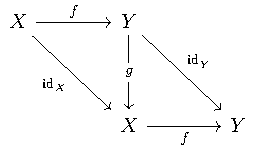
\includegraphics[width=0.3\textwidth]{isomorphism.pdf}}}
                \label{cd: isomorphism}
            \end{equation}
            In other words, $f$ is an isomorphism if there exists a morphism $g$ such that $g \circ f = \textbf{id}_X$ and $f \circ g = \textbf{id}_Y$.

            The morphism $g$ is uniquely determined by $f$ and is called the \emph{inverse} of $f$, denoted as $f^{-1}$.

            Given two objects $X$ and $Y$ in a category $\mathcal{C}$, if there exists an isomorphism from $X$ to $Y$, we say that $X$ and $Y$ are \emph{isomorphic} in $\mathcal{C}$ and write $X \cong Y$.

        \end{definition*}

        [Considering adding examples of isomorphism]
        
        
        \subsection{Terminal object}
        \begin{definition*}[Terminal object]
            Given a category $\mathcal{C}$, an object $T \in \textbf{obj}(\mathcal{C})$ is called a \emph{terminal object} if for all $X \in \textbf{obj}(\mathcal{C})$, there exists a unique \textbf{C}-morphism $f : X \to T$.
        \end{definition*}
        [Considering adding examples of terminal object]

        Terminal objects are unique up to isomorphism. In other words, we have
        \begin{itemize}
            \item 
                if $T$ and $T'$ are both terminal objects in $\mathcal{C}$, then there exists a unique isomorphism $f : T \to T'$.
            \item
                if $T$ is a terminal object in $\mathcal{C}$ and $T \cong T'$, then $T'$ is also a terminal object in $\mathcal{C}$.
        \end{itemize}

        % \subsection{Initial object}
        % \begin{definition*}[Initial object]
        %     Given a category $\mathcal{C}$, an object $I \in \textbf{obj}(\mathcal{C})$ is called an \emph{initial object} if for all $X \in \textbf{obj}(\mathcal{C})$, there exists a unique \textbf{C}-morphism $f : I \to X$.
        % \end{definition*}
        % Initial object is dual to terminal object. By the principle of duality, initial objects are unique up to isomorphism. In other words, we have
        % \begin{itemize}
        %     \item 
        %         if $I$ and $I'$ are both initial objects in $\mathcal{C}$, then there exists a unique isomorphism $f : I \to I'$.
        %     \item
        %         if $I$ is an initial object in $\mathcal{C}$ and $I \cong I'$, then $I'$ is also an initial object in $\mathcal{C}$.
        % \end{itemize}

        
        \subsection{Binary product}
        \begin{definition*}[Binary product]
            Given a category $\mathcal{C}$, the \emph{binary product} of two objects $X$ and $Y$ in $\mathcal{C}$ is specified by
            \begin{itemize}
                \item a $\mathcal{C}$-object $X \times Y$;
                \item two $\mathcal{C}$-morphisms $\pi_1 : X \times Y \to X$ and $\pi_2 : X \times Y \to Y$ called the \emph{projections} of $X \times Y$;
            \end{itemize}
            such that for all $Z \in \textbf{obj}(\mathcal{C})$ and morphisms $f : Z \to X$ and $g : Z \to Y$, there exists a unique morphism $u : Z \to X \times Y$ such that the following diagram commutes in $\mathcal{C}$:
            \begin{equation}
                \vcenter{\hbox{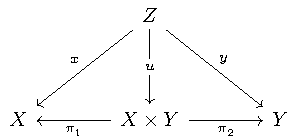
\includegraphics[width=0.4\textwidth]{binary_product.pdf}}}
                \label{cd: binary_product}
            \end{equation}
            The unique morphism $u$ is written as 
            \[ \langle x, y \rangle : Z \to X \times Y \]
            where $x = \pi_1 \circ u$ and $y = \pi_2 \circ u$.
        \end{definition*}
        It can be shown that the binary product is unique up to (unique) isomorphism.


        \subsection{Exponential}
        \begin{definition*}[Exponential]
            Given a category $\mathcal{C}$ with binary products, the \emph{exponential} of two objects $X$ and $Y$ in $\mathcal{C}$ is specified by
            \begin{itemize}
                \item a $\mathcal{C}$-object $X \Rightarrow Y$;
                \item a $\mathcal{C}$-morphism $\textbf{app} : (X \Rightarrow Y) \times X \to Y$ called the \emph{application} of $X \Rightarrow Y$;
            \end{itemize}
            such that for all $Z \in \textbf{obj}(\mathcal{C})$ and morphisms $f : Z \times X \to Y$, there exists a unique morphism $u : Z \to X \Rightarrow Y$ such that the following diagram commutes in $\mathcal{C}$:
            \begin{equation}
                \vcenter{\hbox{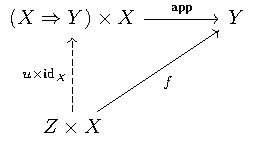
\includegraphics[width=0.4\textwidth]{exponential.pdf}}}
                \label{cd: exponential}
            \end{equation}
            We write $\textbf{cur} f$ for the unique morphism $u$ such that $f = \textbf{app} \circ (\textbf{cur} f \times \textbf{id}_X)$, 
            where $\textbf{cur} f$ is called the \emph{currying} of $f$.
        \end{definition*}
        It can be shown that the exponential is unique up to (unique) isomorphism.

    
        \subsection{Cartesian closed category}
        \begin{definition*}[Cartesian closed category]
            A category $\mathcal{C}$ is called a \emph{Cartesian closed category} (ccc) if it has a terminal object, binary products and exponentials of any two objects.
        \end{definition*}

        
        \subsection{Functor}
        \begin{definition*}[Functor]
            Given two categories $\mathcal{C}$ and $\mathcal{D}$, a \emph{functor} $F: \mathcal{C} \to \mathcal{D}$ is specified by:
            \begin{itemize}
                \item 
                    a function 
                    \[\begin{aligned}
                        \textbf{obj}(\mathcal{C}) &\to \textbf{obj}(\mathcal{D}) \\
                        X &\mapsto F(X)
                    \end{aligned}\]

                \item 
                    for each $X, Y \in \textbf{obj}(\mathcal{C})$, a function 
                    \[\begin{aligned}
                        \mathcal{C}{(X,Y)} &\to \mathcal{D}{(F(X),F(Y))} \\
                        f &\mapsto F(f)
                    \end{aligned}\]
            \end{itemize}
            satisfying the following properties:
            \begin{itemize}
                \item 
                    for all $X, Y \in \textbf{obj}(\mathcal{C})$ and $f \in \mathcal{C}{(X,Y)}$, we have:
                    \begin{equation} \label{law: functor_id}
                        F(\textbf{id}_X) = \textbf{id}_{F(X)}
                    \end{equation}
                \item
                    for all $X, Y, Z \in \textbf{obj}(\mathcal{C})$ and $f \in \mathcal{C}{(X,Y)}$, $g \in \mathcal{C}{(Y,Z)}$, we have:
                    \begin{equation} \label{law: functor_comp}
                        F(g \circ f) = F(g) \circ F(f)
                    \end{equation}
            \end{itemize}
        \end{definition*}

        [Considering adding examples of functors: e.g. free functor, forgetful functor, etc.]

        
        \subsection{Natural transformation}
        \begin{definition*}[Natural transformation]

            Given two categories $\mathcal{C}$ and $\mathcal{D}$, and two functors $F,G: \mathcal{C} \to \mathcal{D}$, a \emph{natural transformation} $\theta : F \to G$ is a family of morphisms $\theta_X \in \mathcal{D}{(F(X),G(X))}$ for each $X \in \textbf{obj}(\mathcal{C})$ such that for all $X, Y \in \textbf{obj}(\mathcal{C})$ and $f \in \mathcal{C}{(X,Y)}$, the following diagram 
            \begin{equation}
                \vcenter{\hbox{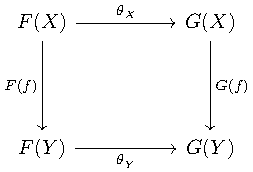
\includegraphics[width=0.3\textwidth]{natural_transformation.pdf}}}
                \label{cd: natural_transformation}
            \end{equation}
            
            commutes in $\mathcal{D}$, i.e. the following equation holds:
            \begin{equation} \label{law: natural_transformation}
                G(f) \circ \theta_X = \theta_Y \circ F(f)
            \end{equation}

        \end{definition*}

        [Considering adding examples of natural transformations]

        
        \subsection{Functor category}
        \begin{definition*}[Functor category]
            Given two categories $\mathcal{C}$ and $\mathcal{D}$, the \emph{functor category} $\mathcal{D}^{\mathcal{C}}$ is the category satisfying the following:
            \begin{itemize}
                \item 
                    the objects of $\mathcal{D}^{\mathcal{C}}$ are all functors $\mathcal{C} \to \mathcal{D}$;
                \item 
                    given two functors $F,G: \mathcal{C} \to \mathcal{D}$, the morphisms from $F$ to $G$ in $\mathcal{D}^{\mathcal{C}}$ are all natural transformations $\theta : F \to G$;
                \item
                    composition and identity morphisms in $\mathcal{D}^{\mathcal{C}}$ are defined as follows:
                    \begin{itemize}
                        \item 
                            the identity morphism $\textbf{id}_F$ on $F$ is defined as $\theta_X = \textbf{id}_{F(X)}$ for all $X \in \textbf{obj}(\mathcal{C})$;
                        \item
                            the composition of two natural transformations $\theta : F \to G$ and $\phi : G \to H$ is defined as $(\phi \circ \theta)_X = \phi_X \circ \theta_X$ for all $X \in \textbf{obj}(\mathcal{C})$.
                    \end{itemize}
            \end{itemize}
        \end{definition*}

        \subsection{Presheaf category}
        \begin{definition*}[Presheaf]
            Given a category $\mathcal{C}$, a \emph{presheaf} on $\mathcal{C}$ is a functor $F: \mathcal{C}^{\textbf{op}} \to \textbf{Set}$.
            A presheaf is a contravariant functor, which means that it reverses the direction of morphisms.
            In other words, a presheaf is a functor that takes objects in $\mathcal{C}$ and assigns them sets, and takes morphisms in $\mathcal{C}$ and assigns them functions between the corresponding sets.
            The presheaf $F$ is defined as follows:
            \begin{itemize}
                \item 
                    for each $X \in \textbf{obj}(\mathcal{C})$, $F(X)$ is a set;
                \item
                    for each $X, Y \in \textbf{obj}(\mathcal{C})$ and $f \in \mathcal{C}{(X,Y)}$, $F(f)$ is a function $F(Y) \to F(X)$.
            \end{itemize}
        \end{definition*}

        \begin{definition*}[Presheaf category]
            Given a category $\mathcal{C}$, the \emph{presheaf category} $\mathcal{P}(\mathcal{C})$ is the functor category $\mathcal{Set}^{\mathcal{C}^{\textbf{op}}}$.
            \begin{itemize}
                \item 
                    the objects of $\mathcal{P}(\mathcal{C})$ are all presheaves on $\mathcal{C}$;
                \item
                    given two presheaves $F,G: \mathcal{C}^{\textbf{op}} \to \mathcal{Set}$, the morphisms from $F$ to $G$ in $\mathcal{P}(\mathcal{C})$ are all natural transformations $\theta : F \to G$.
            \end{itemize}
        \end{definition*}



        \subsection{Yoneda lemma}
        \begin{definition*}[Yoneda functor]
            Given a category $\mathcal{C}$, the \emph{Yoneda functor} $\yo: \mathcal{C} \to \mathcal{Set}^{\mathcal{C}^{\textbf{op}}}$ is defined as follows:
            \begin{itemize}
                \item 
                    for each $X \in \textbf{obj}(\mathcal{C})$, $\yo(X)$ is the functor $y(X) : \mathcal{C}^{\textbf{op}} \to \mathcal{Set}$ defined as:
                    \begin{equation} \label{eq: yoneda_element}
                        \yo(X)(Y) = \mathcal{C}{(Y,X)}
                    \end{equation}
                    for all $Y \in \textbf{obj}(\mathcal{C})$;
                \item
                    for each $X, Y \in \textbf{obj}(\mathcal{C})$ and $f \in \mathcal{C}{(X,Y)}$, $\yo(f)$ is the morphism $\yo(X) \to \yo(Y)$ defined a natural transformation whose component at any given $Z \in \mathcal{C}^{\textbf{op}}$ is given by:
                    \begin{equation} \label{eq: yoneda_morphism}
                        \begin{aligned}
                            (\yo(f))_Z : \mathcal{C}{(Z,Y)} &\to \mathcal{C}{(Z,X)} \\
                            g &\mapsto g \circ f
                        \end{aligned}
                    \end{equation}
                    for all $Z \in \textbf{obj}(\mathcal{C})$.
                \end{itemize}

        \end{definition*}

        \begin{theorem*}[Yoneda lemma]
            Given a category $\mathcal{C}$, the \emph{Yoneda lemma} states that for each object $X \in \textbf{obj}(\mathcal{C})$ and any functor $F: \mathcal{C} \to \textbf{Set}$, there is a natural isomorphism:
            \begin{equation} \label{eq: yoneda_lemma}
                \mathcal{Set}^{\mathcal{C}^{\textbf{op}}}(\yo(X), F) \cong F(X)
            \end{equation}
        \end{theorem*}



        \subsection{Cartesian closed structure in presheaf categories}
        \begin{theorem*}[Cartesian closed structure in presheaf categories]
            Given a small category $\mathcal{C}$, the presheaf category $\mathcal{Set}^{\mathcal{C}^{\textbf{op}}}$ is a Cartesian closed category.
            \begin{itemize}
                \item 
                    The terminal object in $\mathcal{Set}^{\mathcal{C}^{\textbf{op}}}$ is the constant functor $\mathbf{1} : \mathcal{C}^{\textbf{op}} \to \mathcal{Set}$, given by 
                    \begin{equation}
                        \begin{cases}
                            \mathbf{1}(X) = \{\ast\} & \text{for all } X \in \textbf{obj}(\mathcal{C}) \\
                            \mathbf{1}(f) = \textbf{id}_{\{\ast\}} & \text{for all } f \in \mathcal{C}{(X,Y)}
                        \end{cases}
                    \end{equation}

                \item
                    The binary product in $\mathcal{Set}^{\mathcal{C}^{\textbf{op}}}$ is given by the product of functors, which is defined as follows:
                    \begin{equation}
                        \begin{aligned}
                            (F \times G)(X) &= F(X) \times G(X) \\
                            (F \times G)(f) &= F(f) \times G(f)
                        \end{aligned}
                    \end{equation}

                \item
                    The exponential in $\mathcal{Set}^{\mathcal{C}^{\textbf{op}}}$ is given by the Yoneda lemma,
                    \begin{equation}
                        \begin{aligned}
                            G^{F}(X) &= \mathcal{Set}^{\mathcal{C}^{\textbf{op}}}(\yo(X) \times F, G) \\
                            G^{F}(f)(\theta) &= \theta \circ (\yo(f) \times \textbf{id}_F) \quad \text{for all } \theta \in \mathcal{Set}^{\mathcal{C}^{\textbf{op}}}(\yo(Y) \times F, G)
                        \end{aligned}
                    \end{equation}
            \end{itemize}
        \end{theorem*}
        


    \section{Agda}
        \subsection{Basic datatypes and pattern matching}
        We will go through a simple example in PLFA \cite{plfa} to illustrate the basic datatypes and pattern matching in Agda.

        \[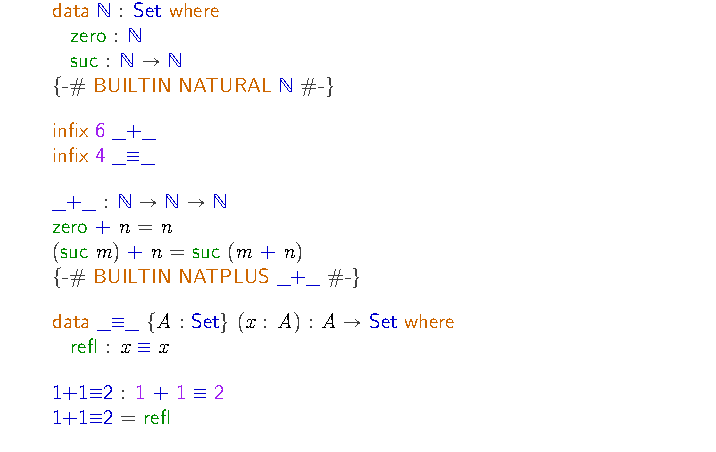
\includegraphics[width=\textwidth]{example.pdf}\]

        Here we define a datatype $\mb{\bN}$ for natural numebers. $\mb{\bN}$ itself has a type $\mb{\mathsf{Set}}$, which is the type of all small types. The natural number is defined as a recursive datatype with two constructors: $\gn{\mathsf{zero}}$ and $\gn{\mathsf{suc}}$, where 
        $\gn{\mathsf{zero}}$ is the base case and $\gn{\mathsf{suc}}$ is the inductive case. The $\gn{\mathsf{zero}}$ constructor has type $\mb{\bN}$, and the $\gn{\mathsf{suc}}$ constructor has type $\mb{\bN \to \bN}$.

        In order to define the plus function $\mb{\_+\_}$, we use pattern matching to match the input argument with the constructors of the datatype. The first case is the base case, where we match the input argument with $\gn{\mathsf{zero}}$. In this case, we return the second argument. The second case is the inductive case, where we match the input argument with $\gn{\mathsf{suc}}$. In this case, we return $\gn{\mathsf{suc}}$ applied to the result of adding one to the second argument.

        \subsection{Dependent Types}
        A dependent type is a type that depends on a value. In terms of type judgement, simple types are in form of
        \[ x_1 : T_1, x_2 : T_2, \dots, x_n : T_n \vdash t(x_1, \dots, x_n) : T \]
        In contrast, dependent types are in form of
        \[ x_1 : T_1, x_2 : T_2, \dots, x_n : T_n \vdash t(x_1, \dots, x_n) : T(x_1, \dots, x_n) \]
        or more generally
        \[ x_1 : T_1, x_2 : T_2(x_1), \dots, x_n : T_n(x_1, \dots, x_{n-1}) \vdash t(x_1, \dots, x_n) : T(x_1, \dots, x_n) \]

        A classical example of dependent types in Agda is the type of vectors, which are lists with a length. 

        \[
\includegraphics[width=\textwidth]{vector.pdf}\]

        Here we define a datatype $\mb{\mathsf{Vec}}$ for vectors. The type of vectors is dependent on the length of the vector. With dependent types, we can encode properties directly into types and ensure that they are satisfied at compile time.

        \subsection{Curry-Howard-Lambek correspondence} \label{subsec: curry-howard-lambek}
        As introduced in \secref{sec: cat}, Curry-Howard correspondence states that there is a correspondence between logic and type theory, and Lambek extended this correspondence to show that cartesian closed categories provide a natural semantic setting for the simply typed lambda calculus. They can be summarised as follows:
        \begin{table}[htb!]
            \centering
            \begin{tabular}{|c|c|c|}
                \hline
                \textbf{Logic} & \textbf{Type theory} & \textbf{Category theory} \\
                \hline
                Proposition & Type & Object \\
                Proof & Term & Morphism \\
                Falsity & Empty type & Initial object \\
                Truth & Unit type & Terminal object \\
                Implication & Function type & Exponential object \\
                Conjunction & Product type & Product \\
                Disjunction & Sum type & Coproduct \\
                Universal quantification & Dependent product type &  \\
                Existential quantification & Dependent sum type &  \\
                \hline
            \end{tabular}
            \caption{Curry-Howard-Lambek correspondence}
            \label{tab: curry-howard-lambek}
        \end{table}

        \subsection{Equality, congruence and substitution}
        Equality here refers to the propositional equality. In Agda it is defined as
        \[
\includegraphics[width=\textwidth]{equality.pdf}\]
        With equality as a type, whenever we want to prove that two terms are equal, we need to provide a witness of the equality. For example if we want to prove $x \equiv y$, we write out a term of type $\mb{\mathsf{x = y}}$, and then give its definition, which constructs a proof of the equality. A simple proof that directly uses the definition of equality is as follows:
        \[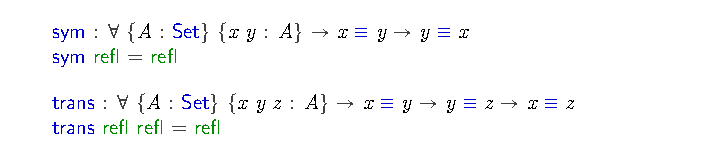
\includegraphics[width=\textwidth]{sym_trans.pdf}\]
        Here we are able to prove the symmetry and transitivity of equality by using the definition of equality. Those two properties are very useful for later proofs. 

        We can also have more complex proof with congruence and substitution, which can also be directly derived from the definition of equality as follows:
        \[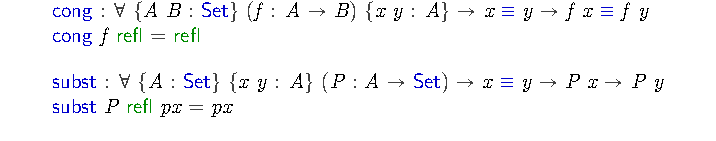
\includegraphics[width=\textwidth]{cong_subst.pdf}\]
        Congruence is a property of equality that states that if two terms are equal, then they can be substituted for each other in any context. Substitution is a property where we can get a new proof by replacing a term in a proof with another term that is equal to it. 

        Here is a simple example of how congruence can be used in a proof:
        \[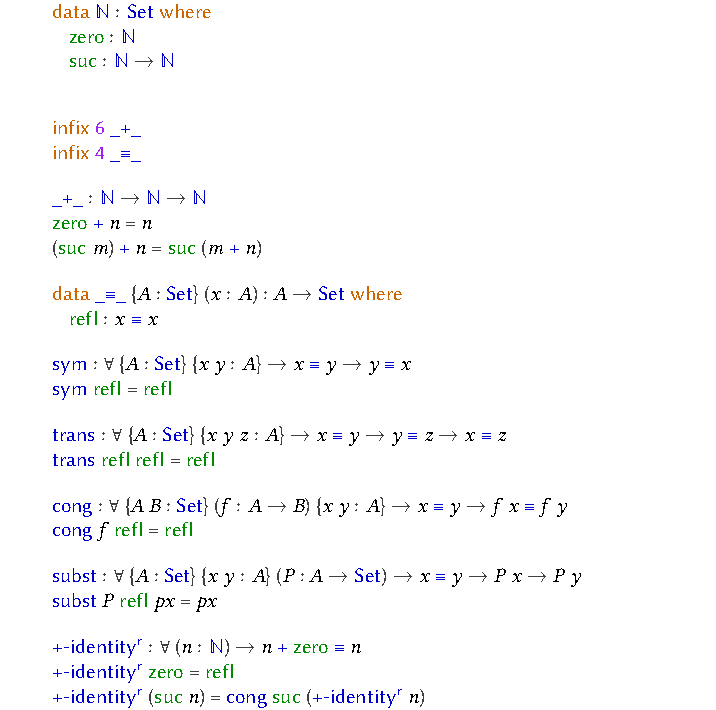
\includegraphics[width=\textwidth]{cong_example.pdf}\]

        In this example, we want to prove that $\gn{\mathsf{zero}}$ is the right identity of the plus function. We do an inductive proof by pattern matching on the first argument of the plus function. 
        
        In the base case, we have $\gn{\mathsf{zero}} \mb{{}+{}} \gn{\mathsf{zero}} \equiv \gn{\mathsf{zero}}$, which is trivially true by the definition of the plus function (zero is defined to be the left identity of the plus function). 
        
        In the inductive case, we need to show $\gn{\mathsf{suc}}\ n \mb{{}+{}} \gn{\mathsf{zero}} \equiv \gn{\mathsf{suc}}\ n$. We can use the definition of the plus function to rewrite the left-hand side as $\gn{\mathsf{suc}}\ (n \mb{{}+{}} \gn{\mathsf{zero}})$. By the inductive hypothesis, we know that $n \mb{{}+{}} \gn{\mathsf{zero}} \equiv n$, so we can substitute $n$ for $n \mb{{}+{}} \gn{\mathsf{zero}}$ in the right-hand side by congruence, and we are done.

        \subsection{Proof Example}
        [decide exact example here]

        \subsection{Standard library}
        The Agda standard library \cite{agda_std} is a collection of modules that provide a wide range of useful functions and types. It includes modules for basic data types, such as natural numbers, lists, and vectors. In my implementation, however, I defined most of the basic data types and functions from scratch for the following two reasons:
        \begin{itemize}
            \item
                I wanted to have a better understanding of the basic data types and functions, so I decided to implement them from scratch.
            \item
                I need a particular representation of minus operation that ensures the input is always valid. This is further explained in [to add]
        \end{itemize}
        
        With standard library, we can use actual numbers $1, 2, 3, \dots$ instead of calling the constructor $\gn{\mathsf{suc}}$ multiple times. This is a convenient feature for testing. Agda provides a way to link self-defined functions to the standard library with a BUILTIN programa. This allows me to use a convenient syntax for numbers, while still using the self-defined functions in the implementation.

        
        \subsection{Interactive programming with holes} \label{subsec: holes}
        A feature of Agda is that it allows us to write programs with holes interatively. A hole is a placeholder for a term that we have not yet defined. By leaving holes in place of undefined terms, we can write programs that are incomplete but still type-check, and Agda's type checker will guide completion of the program: the context window displays inferred types of the holes, available variables and candidate terms with their types. Holes also supports case split and refinement, which means we can fill in a hole partially and split it into smaller holes. 

        [Considering adding examples of holes and case split, see https://plfa.github.io/Naturals/]

        In my implementation, I used holes to write the terms in the compiler. The complex terms are incrementally filled and verified by interatively refining partial implementations, reducing post-hoc debugging and ensuring robustness.


    \section{Requirement Analysis}
    To complete a compiler in Agda we need to implement the following components:
    \begin{itemize}
        \item 
            A file source.agda that record the syntax of the source language.

        \item
            A file target.agda that record the syntax of the target language.

        \item
            A file compiler.agda that uses source.agda and target.agda as modules, and write functions whose input is a term in the source language and output is a term in the target language.
    \end{itemize}
    The success criteria of the project is that the compiler can compile a term in the source language to a term in the target language, and the output term is well-typed in the target language.


    \section{Tools Used}
    Completing the project is an iterative process. I used Git \cite{git} for version control, and work had been synchronised with a GitHub \cite{github} repository for backup.

    For the development environment, I tried both Emacs \cite{emacs} and Visual Studio Code \cite{vscode} with an agda-mode extension \cite{agda_mode} on Windows Subsystem for Linux with Ubuntu \cite{wsl_ubuntu} 22.04 LTS. I am more familiar with the snippet and syntax highlighting features of Visual Studio Code, so I used it for most of the development. 

    Code from the PLFA tutorial and Agda standard library \cite{agda_std} were used as references. 

    \section{Summary}
    \begin{itemize}
        \item 
        requirement Analysis

        \item
        tools and engineering approach

    \end{itemize}

\chapter{Implementation}

\chapter{Evaluation}

\chapter{Conclusion}

    \printbibliography

\end{document}